\begin{frame}
  \frametitle{Valgrind (1)}
  \begin{columns}[T]
    \column{0.8\textwidth}
    \url{https://valgrind.org/}
    \begin{itemize}
    \item GNU GPL Software suite for debugging and profiling programs.
    \item Supported platforms: Linux on x86, x86\_64, arm (armv7 only),
      arm64, mips32, s390, ppc32 and ppc64. Also supported on other
      operating systems (Android, Darwin, Illumos, Solaris...)
    \item Can detect many memory management and threading bugs.
    \item Profiler: provides information helpful to speed up your
      program and reduce its memory usage.
    \item The most popular tool for this usage. Even used by projects
      with hundreds of programmers.
    \end{itemize}
    \column{0.2\textwidth}
    
\includegraphics[width=\textwidth]{slides/sysdev-application-development/valgrind1.png}
  \end{columns}
\end{frame}

\begin{frame}
  \frametitle{Valgrind (2)}
  \begin{columns}[T]
    \column{0.8\textwidth}
    \begin{itemize}
    \item Can be used to run any program, without the need to
      recompile it.
    \item Examples\\
      \small
      \code{valgrind --leak-check=yes <program>} (leak check mode)\\
      \code{valgrind --tool=callgrind --dump-instr=yes --simulate-cache=yes --collect-jumps=yes <program>} (profiling mode)
      \normalsize
    \item Works by adding its own instrumentation to your code and
      then running in on its own virtual cpu core. Significantly slows
      down execution, but still fine for debugging and profiling!
    \item More details on \url{https://valgrind.org/info/} and
      \url{https://valgrind.org/docs/manual/manual.html}
    \item The Valgrind tool suite is easy to add to your root filesystem
          with Buildroot.
    \end{itemize}
    \column{0.2\textwidth}
    
\includegraphics[width=\textwidth]{slides/sysdev-application-development/valgrind2.png}
  \end{columns}
\end{frame}

\begin{frame}
  \frametitle{Kcachegrind - Visualizing Valgrind profiling data}
    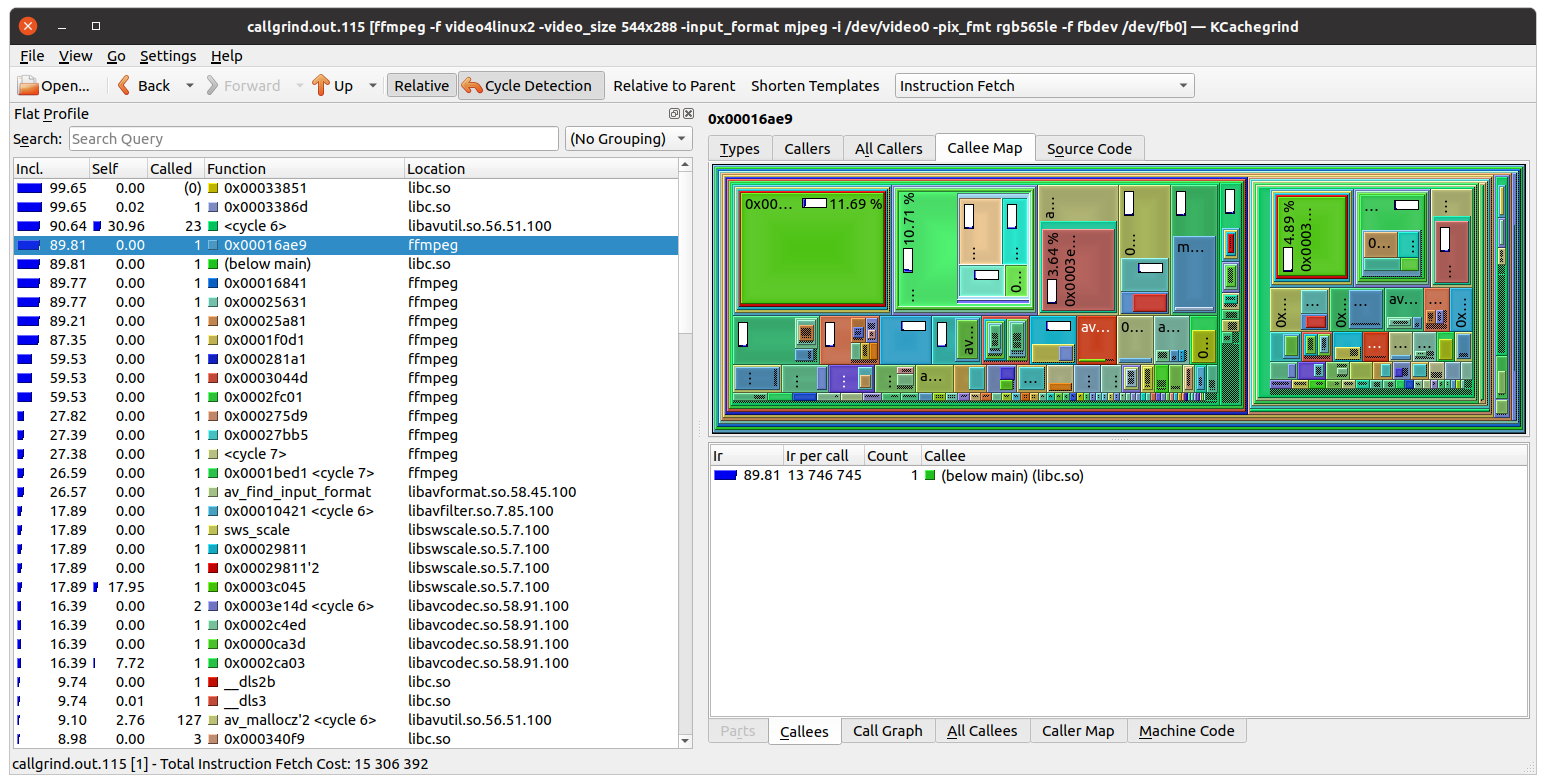
\includegraphics[width=\textwidth]{common/kcachegrind.png}
    \small Directly run it on Callgrind's output file.
\end{frame}
